\documentclass{beamer}

%\usepackage[table]{xcolor}
\mode<presentation> {
  \usetheme{Boadilla}
%  \usetheme{Pittsburgh}
%\usefonttheme[2]{sans}
\renewcommand{\familydefault}{cmss}
%\usepackage{lmodern}
%\usepackage[T1]{fontenc}
%\usepackage{palatino}
%\usepackage{cmbright}
  \setbeamercovered{transparent}
\useinnertheme{rectangles}
}
%\usepackage{normalem}{ulem}
%\usepackage{colortbl, textcomp}
\setbeamercolor{normal text}{fg=black}
\setbeamercolor{structure}{fg= black}
\definecolor{trial}{cmyk}{1,0,0, 0}
\definecolor{trial2}{cmyk}{0.00,0,1, 0}
\definecolor{darkgreen}{rgb}{0,.4, 0.1}
\usepackage{array}
\newcommand{\argmin}{\arg\!\min}
\beamertemplatesolidbackgroundcolor{white}  \setbeamercolor{alerted
text}{fg=red}

\setbeamertemplate{caption}[numbered]\newcounter{mylastframe}

%\usepackage{color}
\usepackage{tikz}
\usetikzlibrary{arrows}
\usepackage{colortbl}
%\usepackage[usenames, dvipsnames]{color}
%\setbeamertemplate{caption}[numbered]\newcounter{mylastframe}c
%\newcolumntype{Y}{\columncolor[cmyk]{0, 0, 1, 0}\raggedright}
%\newcolumntype{C}{\columncolor[cmyk]{1, 0, 0, 0}\raggedright}
%\newcolumntype{G}{\columncolor[rgb]{0, 1, 0}\raggedright}
%\newcolumntype{R}{\columncolor[rgb]{1, 0, 0}\raggedright}

%\begin{beamerboxesrounded}[upper=uppercol,lower=lowercol,shadow=true]{Block}
%$A = B$.
%\end{beamerboxesrounded}}
\renewcommand{\familydefault}{cmss}
%\usepackage[all]{xy}

\usepackage{tikz}
\usepackage{lipsum}

 \newenvironment{changemargin}[3]{%
 \begin{list}{}{%
 \setlength{\topsep}{0pt}%
 \setlength{\leftmargin}{#1}%
 \setlength{\rightmargin}{#2}%
 \setlength{\topmargin}{#3}%
 \setlength{\listparindent}{\parindent}%
 \setlength{\itemindent}{\parindent}%
 \setlength{\parsep}{\parskip}%
 }%
\item[]}{\end{list}}
\usetikzlibrary{arrows}
%\usepackage{palatino}
%\usepackage{eulervm}
\usecolortheme{lily}
\newtheorem{com}{Comment}
\newtheorem{lem} {Lemma}
\newtheorem{prop}{Proposition}
\newtheorem{thm}{Theorem}
\newtheorem{defn}{Definition}
\newtheorem{cor}{Corollary}
\newtheorem{obs}{Observation}
 \numberwithin{equation}{section}

%\usepackage[latin1]{inputenc}
\title[Text as Data] % (optional, nur bei langen Titeln nötig)
{Text as Data}

\author{Justin Grimmer}
\institute[Stanford University]{Associate Professor\\Department of Political Science \\  Stanford University}
\vspace{0.3in}


\date{October 30th, 2014}%[Big Data Workshop] 
%\date{\today}


\begin{document}
\begin{frame}
\titlepage
\end{frame}


\begin{frame}
\frametitle{Structured Topic Models}

\begin{itemize}
\item[1)] Task: 
\begin{itemize}
\item[-] Examine how document attention, topic content varies$\leadsto$ over time, across authors, or with \alert{general set of covariates}
\end{itemize}
\item[2)] Objective Function
\begin{eqnarray}
&& f(\boldsymbol{X}, \boldsymbol{\pi}, \boldsymbol{\Theta}, \boldsymbol{\alpha}, \alert{\boldsymbol{W}})  \nonumber 
\end{eqnarray}
Where:
\begin{itemize}
\item[-] $\boldsymbol{W}$ condition on information in document$\leadsto$ other potential modifications to objective function.  \alert{Meta-data}.  
\item[-] $f(\boldsymbol{X}, \boldsymbol{\pi}, \boldsymbol{\Theta}, \boldsymbol{\alpha}, \alert{\boldsymbol{W}})$ may encode additional information$\leadsto$ layers of clustering, layers of topics, etc
\end{itemize}
\item[3)] Optimization
\begin{itemize}
\item[-] EM, Variational Approximation, Gibbs Sampling, $\hdots $
\end{itemize}
\item[4)] Validation$\leadsto$ many of the same methods from clustering
\begin{itemize}
\item[-] Semantic, Convergent, Discriminant, Predictive, Hypothesis validity
\item[-] \alert{How do we avoid the electric machine critique}?
\end{itemize}
\end{itemize}

\end{frame}



\begin{frame}
\frametitle{LDA Revisited}


\only<1>{\begin{eqnarray}
\boldsymbol{\theta}_{k} & \sim & \text{Dirichlet}(\boldsymbol{1}) \nonumber \\
\boldsymbol{\pi}_{i}|\boldsymbol{\alpha} & \sim &  \text{Dirichlet}(\boldsymbol{\alpha}) \nonumber \\
\boldsymbol{\tau}_{im}| \boldsymbol{\pi}_{i} & \sim & \text{Multinomial}(1, \boldsymbol{\pi}_{i}) \nonumber \\
x_{im} | \boldsymbol{\theta}_{k}, \tau_{imk} = 1 & \sim & \text{Multinomial}(1, \boldsymbol{\theta}_{k}) \nonumber 
\end{eqnarray}}

\only<2>{\begin{eqnarray}
\textbf{Unigram Model}_{k} & \sim & \text{Dirichlet}(\boldsymbol{1}) \nonumber \\
\textbf{Doc. Prop}_{i} & \sim & \text{Dirichlet}(\textbf{Pop. Proportion}) \nonumber \\
\textbf{Word Topic}_{im} & \sim & \text{Multinomial}(1, \textbf{Doc. Prop}_{i}) \nonumber \\
\text{Word}_{im} & \sim & \text{Multinomial}(1, \textbf{Unigram Model}_{k}) \nonumber 
\end{eqnarray}}







\end{frame}



\begin{frame}
\frametitle{A General Hierarchical Structure} 

LDA: 
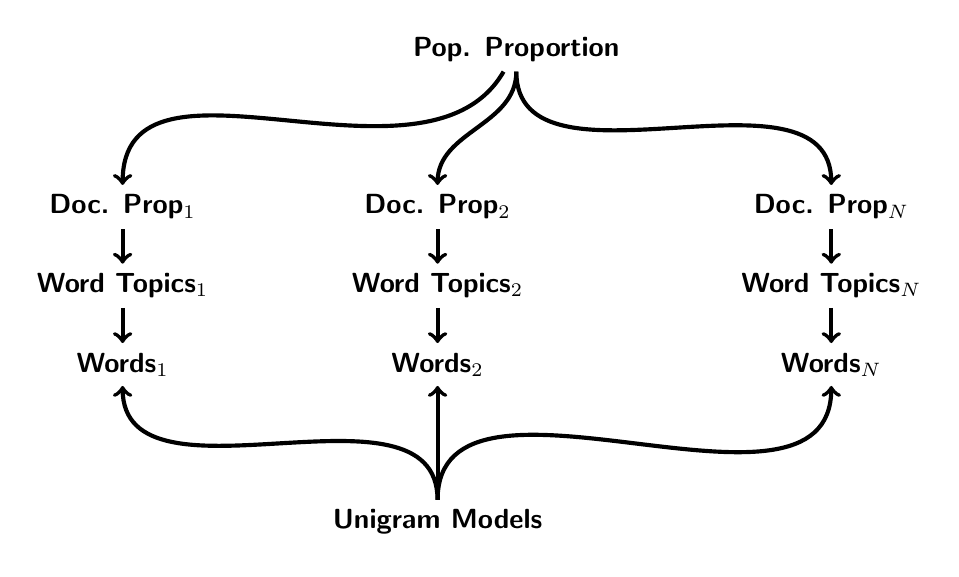
\begin{tikzpicture}

\node (col) at (0, 10) [] {\textbf{Pop. Proportion}} ; 

\invisible<1>{



\node (doc1) at (-5, 8) [] {\textbf{Doc. Prop}$_{1}$} ; 
\node (doc2) at (-1, 8) [] {\textbf{Doc. Prop}$_{2}$} ; 
\node (dots) at ( 2, 8) [] {$\hdots$} ; 
\node (docN) at (4, 8) [] {\textbf{Doc. Prop}$_{N}$} ; 

\draw[->, line width=1.5pt] (col) to [out=240, in = 90] (doc1); 
\draw[->, line width=1.5pt] (col) to [out=270, in = 90] (doc2); 
\draw[->, line width=1.5pt] (col) to [out=270, in = 90] (docN); 

}

\invisible<1-2>{


\node (word11) at (-5, 7) [] {\textbf{Word Topics}$_{1}$} ; 
\node (word22) at (-1, 7) [] {\textbf{Word Topics}$_{2}$} ; 
\node (wordnn) at (4, 7) [] {\textbf{Word Topics}$_{N}$ } ; 

\draw[->, line width=1.5pt] (doc1) to [out=270, in=90] (word11) ; 
\draw[->, line width=1.5pt] (doc2) to [out=270, in=90] (word22) ; 
\draw[->, line width=1.5pt] (docN) to [out=270, in=90] (wordnn) ; 




}



\invisible<1-3>{

\node (wordaa) at (-5, 6) [] {\textbf{Words}$_{1}$} ; 
\node (wordbb) at (-1, 6) [] {\textbf{Words}$_{2}$} ; 
\node (wordcc) at (4, 6) [] {\textbf{Words}$_{N}$ } ; 


\draw[->, line width = 1.5pt] (word11) to [out = 270, in = 90] (wordaa); 
\draw[->, line width = 1.5pt] (word22) to [out = 270, in = 90] (wordbb); 
\draw[->, line width = 1.5pt] (wordnn) to [out = 270, in = 90] (wordcc); 

\node (topics) at (-1, 4) [] {$\textbf{Unigram Models}$} ; 



\draw[->, line width = 1.5pt] (topics) to [out = 90, in = 270] (wordaa); 
\draw[->, line width = 1.5pt] (topics) to [out = 90, in = 270] (wordbb); 
\draw[->, line width = 1.5pt] (topics) to [out = 90, in = 270] (wordcc); 



}


\end{tikzpicture}


\pause \pause \pause 

\end{frame}



\begin{frame}
\frametitle{A General Hierarchical Structure} 

Dynamic Topic Model (Quinn et al 2010) 
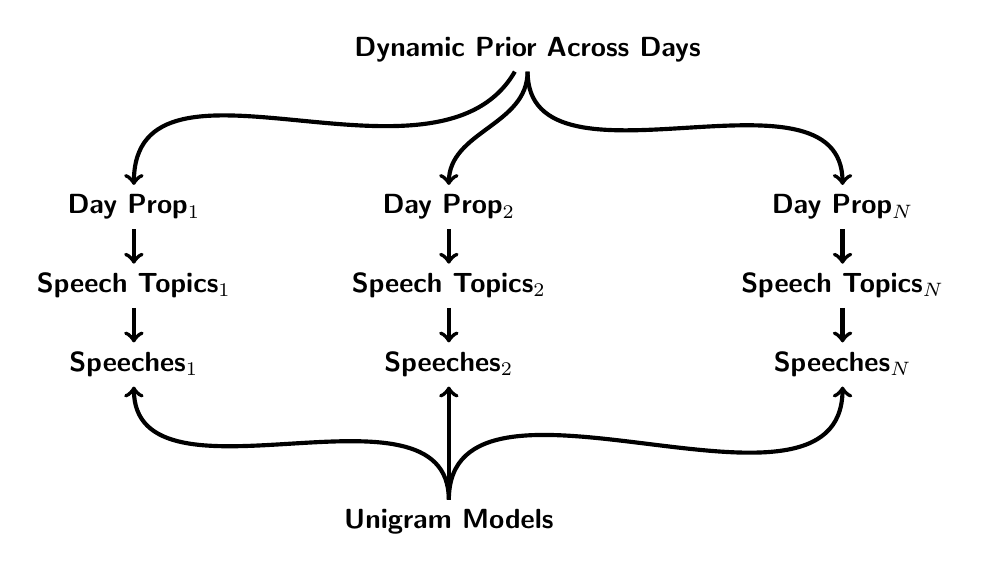
\begin{tikzpicture}

\node (col) at (0, 10) [] {\textbf{Dynamic Prior Across Days}} ; 

\invisible<1>{



\node (doc1) at (-5, 8) [] {\textbf{Day Prop}$_{1}$} ; 
\node (doc2) at (-1, 8) [] {\textbf{Day Prop}$_{2}$} ; 
\node (dots) at ( 2, 8) [] {$\hdots$} ; 
\node (docN) at (4, 8) [] {\textbf{Day Prop}$_{N}$} ; 

\draw[->, line width=1.5pt] (col) to [out=240, in = 90] (doc1); 
\draw[->, line width=1.5pt] (col) to [out=270, in = 90] (doc2); 
\draw[->, line width=1.5pt] (col) to [out=270, in = 90] (docN); 

}

\invisible<1-2>{


\node (word11) at (-5, 7) [] {\textbf{Speech Topics}$_{1}$} ; 
\node (word22) at (-1, 7) [] {\textbf{Speech Topics}$_{2}$} ; 
\node (wordnn) at (4, 7) [] {\textbf{Speech Topics}$_{N}$ } ; 

\draw[->, line width=1.5pt] (doc1) to [out=270, in=90] (word11) ; 
\draw[->, line width=1.5pt] (doc2) to [out=270, in=90] (word22) ; 
\draw[->, line width=1.5pt] (docN) to [out=270, in=90] (wordnn) ; 




}



\invisible<1-3>{

\node (wordaa) at (-5, 6) [] {\textbf{Speeches}$_{1}$} ; 
\node (wordbb) at (-1, 6) [] {\textbf{Speeches}$_{2}$} ; 
\node (wordcc) at (4, 6) [] {\textbf{Speeches}$_{N}$ } ; 


\draw[->, line width = 1.5pt] (word11) to [out = 270, in = 90] (wordaa); 
\draw[->, line width = 1.5pt] (word22) to [out = 270, in = 90] (wordbb); 
\draw[->, line width = 1.5pt] (wordnn) to [out = 270, in = 90] (wordcc); 

\node (topics) at (-1, 4) [] {$\textbf{Unigram Models}$} ; 



\draw[->, line width = 1.5pt] (topics) to [out = 90, in = 270] (wordaa); 
\draw[->, line width = 1.5pt] (topics) to [out = 90, in = 270] (wordbb); 
\draw[->, line width = 1.5pt] (topics) to [out = 90, in = 270] (wordcc); 



}


\end{tikzpicture}


\pause \pause \pause 

\end{frame}




\begin{frame}
\frametitle{A General Hierarchical Structure} 

Expressed Agenda Model (Grimmer 2010) 
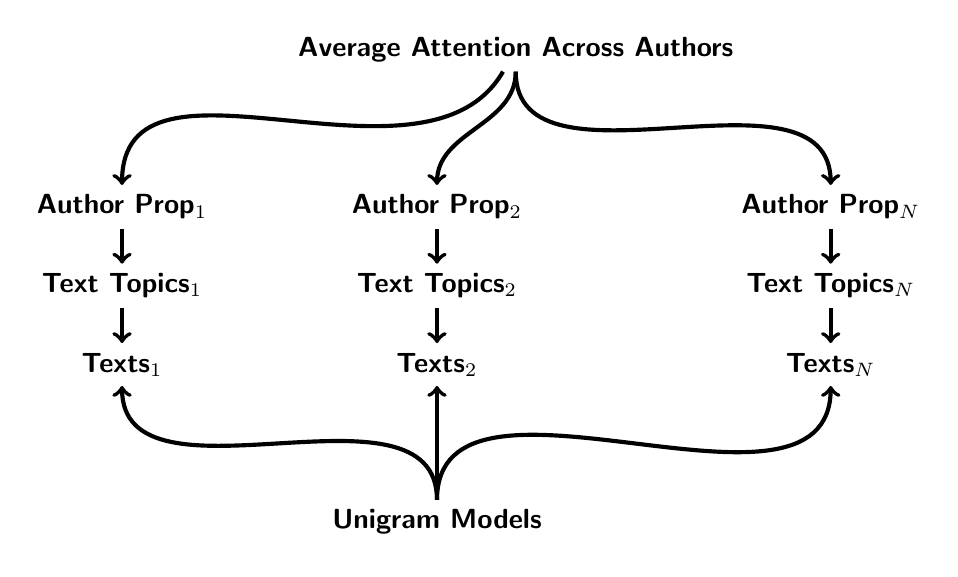
\begin{tikzpicture}

\node (col) at (0, 10) [] {\textbf{Average Attention Across Authors}} ; 

\invisible<1>{



\node (doc1) at (-5, 8) [] {\textbf{Author Prop}$_{1}$} ; 
\node (doc2) at (-1, 8) [] {\textbf{Author Prop}$_{2}$} ; 
\node (dots) at ( 2, 8) [] {$\hdots$} ; 
\node (docN) at (4, 8) [] {\textbf{Author Prop}$_{N}$} ; 

\draw[->, line width=1.5pt] (col) to [out=240, in = 90] (doc1); 
\draw[->, line width=1.5pt] (col) to [out=270, in = 90] (doc2); 
\draw[->, line width=1.5pt] (col) to [out=270, in = 90] (docN); 

}

\invisible<1-2>{


\node (word11) at (-5, 7) [] {\textbf{Text Topics}$_{1}$} ; 
\node (word22) at (-1, 7) [] {\textbf{Text Topics}$_{2}$} ; 
\node (wordnn) at (4, 7) [] {\textbf{Text Topics}$_{N}$ } ; 

\draw[->, line width=1.5pt] (doc1) to [out=270, in=90] (word11) ; 
\draw[->, line width=1.5pt] (doc2) to [out=270, in=90] (word22) ; 
\draw[->, line width=1.5pt] (docN) to [out=270, in=90] (wordnn) ; 




}



\invisible<1-3>{

\node (wordaa) at (-5, 6) [] {\textbf{Texts}$_{1}$} ; 
\node (wordbb) at (-1, 6) [] {\textbf{Texts}$_{2}$} ; 
\node (wordcc) at (4, 6) [] {\textbf{Texts}$_{N}$ } ; 


\draw[->, line width = 1.5pt] (word11) to [out = 270, in = 90] (wordaa); 
\draw[->, line width = 1.5pt] (word22) to [out = 270, in = 90] (wordbb); 
\draw[->, line width = 1.5pt] (wordnn) to [out = 270, in = 90] (wordcc); 

\node (topics) at (-1, 4) [] {$\textbf{Unigram Models}$} ; 



\draw[->, line width = 1.5pt] (topics) to [out = 90, in = 270] (wordaa); 
\draw[->, line width = 1.5pt] (topics) to [out = 90, in = 270] (wordbb); 
\draw[->, line width = 1.5pt] (topics) to [out = 90, in = 270] (wordcc); 



}


\end{tikzpicture}


\pause \pause \pause 

\end{frame}


\begin{frame}
\frametitle{A General Hierarchical Structure} 

Structural Topic Model (Roberts, Stewart, Airoldi 2014) 
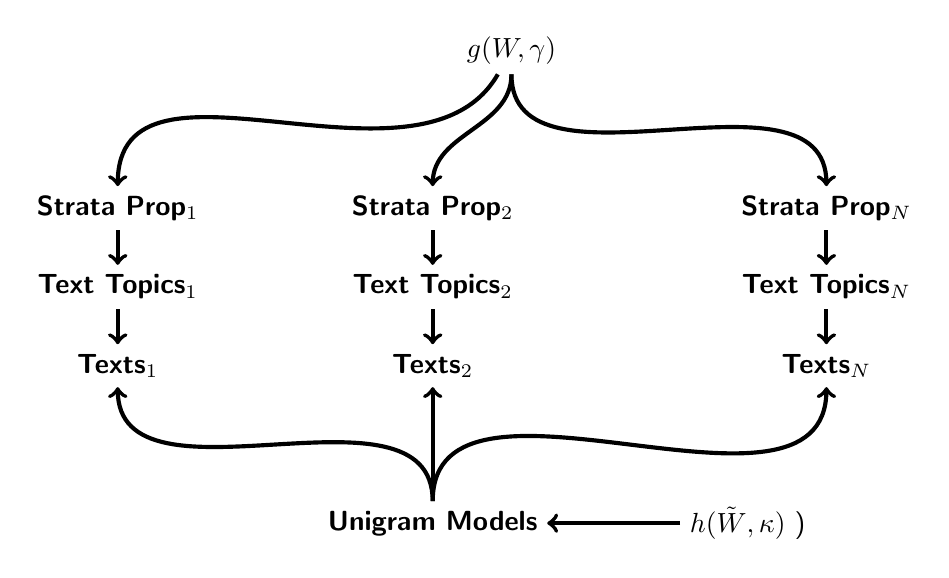
\begin{tikzpicture}

\node (col) at (0, 10) [] {$g(\boldsymbol{W}, \boldsymbol{\gamma}) $} ; 

\invisible<1>{



\node (doc1) at (-5, 8) [] {\textbf{Strata Prop}$_{1}$} ; 
\node (doc2) at (-1, 8) [] {\textbf{Strata Prop}$_{2}$} ; 
\node (dots) at ( 2, 8) [] {$\hdots$} ; 
\node (docN) at (4, 8) [] {\textbf{Strata Prop}$_{N}$} ; 

\draw[->, line width=1.5pt] (col) to [out=240, in = 90] (doc1); 
\draw[->, line width=1.5pt] (col) to [out=270, in = 90] (doc2); 
\draw[->, line width=1.5pt] (col) to [out=270, in = 90] (docN); 

}

\invisible<1-2>{


\node (word11) at (-5, 7) [] {\textbf{Text Topics}$_{1}$} ; 
\node (word22) at (-1, 7) [] {\textbf{Text Topics}$_{2}$} ; 
\node (wordnn) at (4, 7) [] {\textbf{Text Topics}$_{N}$ } ; 

\draw[->, line width=1.5pt] (doc1) to [out=270, in=90] (word11) ; 
\draw[->, line width=1.5pt] (doc2) to [out=270, in=90] (word22) ; 
\draw[->, line width=1.5pt] (docN) to [out=270, in=90] (wordnn) ; 




}



\invisible<1-3>{

\node (wordaa) at (-5, 6) [] {\textbf{Texts}$_{1}$} ; 
\node (wordbb) at (-1, 6) [] {\textbf{Texts}$_{2}$} ; 
\node (wordcc) at (4, 6) [] {\textbf{Texts}$_{N}$ } ; 


\draw[->, line width = 1.5pt] (word11) to [out = 270, in = 90] (wordaa); 
\draw[->, line width = 1.5pt] (word22) to [out = 270, in = 90] (wordbb); 
\draw[->, line width = 1.5pt] (wordnn) to [out = 270, in = 90] (wordcc); 

\node (topics) at (-1, 4) [] {$\textbf{Unigram Models}$} ; 



\draw[->, line width = 1.5pt] (topics) to [out = 90, in = 270] (wordaa); 
\draw[->, line width = 1.5pt] (topics) to [out = 90, in = 270] (wordbb); 
\draw[->, line width = 1.5pt] (topics) to [out = 90, in = 270] (wordcc); 



}

\invisible<1-4>{
\node (reg) at (3, 4) [] {$h(\tilde{\boldsymbol{W}}, \boldsymbol{\kappa})$ )}; 

\draw[->, line width = 1.5pt] (reg) to [out = 180, in = 0] (topics); 

}
\end{tikzpicture}


\pause \pause \pause \pause 

\end{frame}


\begin{frame}
\frametitle{A General Hierarchical Structure} 

Conditioning on Unknown Covariates$\leadsto$ levels of mixtures at proportions (Grimmer 2013; Wallach 2008) 
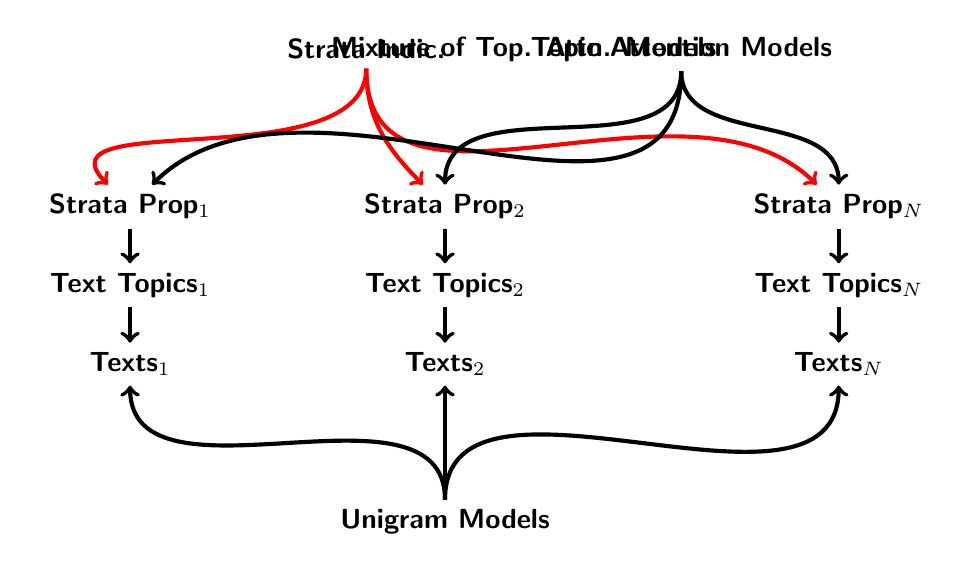
\begin{tikzpicture}

\only<1>{\node (col_on) at (0, 10)[] {\textbf{Mixture of Top. Attn. Models}} ; }

\invisible<1>{\node (col1) at (-2, 10) [] {\textbf{Strata Indic.} } ; 
\node (col) at (2, 10) [] {\textbf{Topic Attention Models} }  ; }

\invisible<1-2>{



\node (doc1) at (-5, 8) [] {\textbf{Strata Prop}$_{1}$} ; 
\node (doc2) at (-1, 8) [] {\textbf{Strata Prop}$_{2}$} ; 
\node (dots) at ( 2, 8) [] {$\hdots$} ; 
\node (docN) at (4, 8) [] {\textbf{Strata Prop}$_{N}$} ; 


\draw[->, line width=1.5pt, red] (col1) to [out=270, in = 135] (doc1); 
\draw[->, line width=1.5pt, red] (col1) to [out=270, in = 135] (doc2); 
\draw[->, line width=1.5pt, red] (col1) to [out=270, in = 135] (docN); 
}

\invisible<1-3>{

\draw[->, line width=1.5pt] (col) to [out=270, in = 45] (doc1); 
\draw[->, line width=1.5pt] (col) to [out=270, in = 90] (doc2); 
\draw[->, line width=1.5pt] (col) to [out=270, in = 90] (docN); 




}

\invisible<1-4>{


\node (word11) at (-5, 7) [] {\textbf{Text Topics}$_{1}$} ; 
\node (word22) at (-1, 7) [] {\textbf{Text Topics}$_{2}$} ; 
\node (wordnn) at (4, 7) [] {\textbf{Text Topics}$_{N}$ } ; 

\draw[->, line width=1.5pt] (doc1) to [out=270, in=90] (word11) ; 
\draw[->, line width=1.5pt] (doc2) to [out=270, in=90] (word22) ; 
\draw[->, line width=1.5pt] (docN) to [out=270, in=90] (wordnn) ; 




}



\invisible<1-5>{

\node (wordaa) at (-5, 6) [] {\textbf{Texts}$_{1}$} ; 
\node (wordbb) at (-1, 6) [] {\textbf{Texts}$_{2}$} ; 
\node (wordcc) at (4, 6) [] {\textbf{Texts}$_{N}$ } ; 


\draw[->, line width = 1.5pt] (word11) to [out = 270, in = 90] (wordaa); 
\draw[->, line width = 1.5pt] (word22) to [out = 270, in = 90] (wordbb); 
\draw[->, line width = 1.5pt] (wordnn) to [out = 270, in = 90] (wordcc); 

\node (topics) at (-1, 4) [] {$\textbf{Unigram Models}$} ; 



\draw[->, line width = 1.5pt] (topics) to [out = 90, in = 270] (wordaa); 
\draw[->, line width = 1.5pt] (topics) to [out = 90, in = 270] (wordbb); 
\draw[->, line width = 1.5pt] (topics) to [out = 90, in = 270] (wordcc); 



}


\end{tikzpicture}


\pause \pause \pause \pause \pause 

\end{frame}



\begin{frame}
\frametitle{A General Hierarchical Structure} 

Conditioning on Unknown Covariates for Topics$\leadsto$ hierarchy of topics (Li and McCallum 2006; Blaydes, Grimmer, and McQueen 2014) 
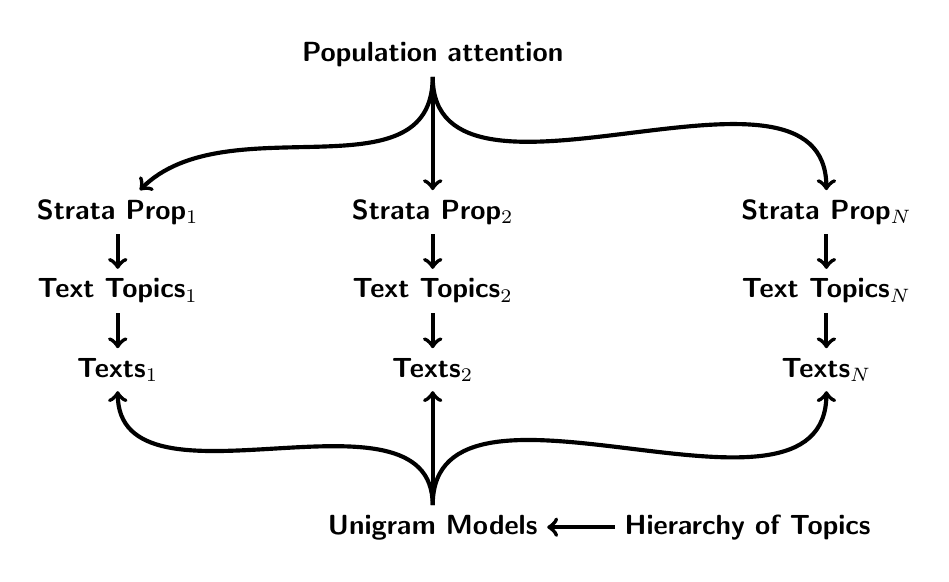
\begin{tikzpicture}

\node (col) at (-1, 10)[] {\textbf{Population attention}} ; 

\invisible<1>{



\node (doc1) at (-5, 8) [] {\textbf{Strata Prop}$_{1}$} ; 
\node (doc2) at (-1, 8) [] {\textbf{Strata Prop}$_{2}$} ; 
\node (dots) at ( 2, 8) [] {$\hdots$} ; 
\node (docN) at (4, 8) [] {\textbf{Strata Prop}$_{N}$} ; 



\draw[->, line width=1.5pt] (col) to [out=270, in = 45] (doc1); 
\draw[->, line width=1.5pt] (col) to [out=270, in = 90] (doc2); 
\draw[->, line width=1.5pt] (col) to [out=270, in = 90] (docN); 




}

\invisible<1-2>{


\node (word11) at (-5, 7) [] {\textbf{Text Topics}$_{1}$} ; 
\node (word22) at (-1, 7) [] {\textbf{Text Topics}$_{2}$} ; 
\node (wordnn) at (4, 7) [] {\textbf{Text Topics}$_{N}$ } ; 

\draw[->, line width=1.5pt] (doc1) to [out=270, in=90] (word11) ; 
\draw[->, line width=1.5pt] (doc2) to [out=270, in=90] (word22) ; 
\draw[->, line width=1.5pt] (docN) to [out=270, in=90] (wordnn) ; 




}



\invisible<1-3>{

\node (wordaa) at (-5, 6) [] {\textbf{Texts}$_{1}$} ; 
\node (wordbb) at (-1, 6) [] {\textbf{Texts}$_{2}$} ; 
\node (wordcc) at (4, 6) [] {\textbf{Texts}$_{N}$ } ; 


\draw[->, line width = 1.5pt] (word11) to [out = 270, in = 90] (wordaa); 
\draw[->, line width = 1.5pt] (word22) to [out = 270, in = 90] (wordbb); 
\draw[->, line width = 1.5pt] (wordnn) to [out = 270, in = 90] (wordcc); 

\node (topics) at (-1, 4) [] {$\textbf{Unigram Models}$} ; 



\draw[->, line width = 1.5pt] (topics) to [out = 90, in = 270] (wordaa); 
\draw[->, line width = 1.5pt] (topics) to [out = 90, in = 270] (wordbb); 
\draw[->, line width = 1.5pt] (topics) to [out = 90, in = 270] (wordcc); 



}

\invisible<1-4>{
\node (mix) at (3, 4) [] {\textbf{Hierarchy of Topics}} ; 
\draw[->, line width = 1.5pt] (mix) to [out = 180, in = 0] (topics); 
}


\end{tikzpicture}


\pause \pause \pause \pause \pause 

\end{frame}

\begin{frame}
\frametitle{Why Encode Structure in Extensions of LDA?}

\pause 

\begin{itemize}
\invisible<1>{\item[-] Substantive reasons} \pause 
\begin{itemize}
\invisible<1-2>{\item[-] Additional structure corresponds to substantively interesting content} \pause 
\invisible<1-3>{\item[-] Avoids potential ad-hoc secondary analysis} \pause 
\invisible<1-4>{\item[-] Clear data generating process} \pause 
\end{itemize}
\invisible<1-5>{\item[-] Statistical reasons} \pause 
\begin{itemize}
\invisible<1-6>{\item[-] \alert{Smoothing}$\leadsto$ borrow information across groups intelligently} \pause 
\invisible<1-7>{\item[-] \alert{Uncertainty}$\leadsto$ potential for better uncertainty estimates} \pause 
\invisible<1-8>{\item[-] \alert{Improved topics}$\leadsto$ small word conditions, structure could help} 
\end{itemize}
\end{itemize}





\end{frame}




\begin{frame}
\frametitle{Plan for the Class}

\begin{itemize}
\item[1)] Discuss model with unknown covariates for strata proportions$\leadsto$ presentational style
\item[2)] Discuss model with hierarchy of topics$\leadsto$ mirrors genre
\end{itemize}


\end{frame}



\begin{frame}
\frametitle{Unknown Covariates for Issue Attention: Measuring Attention in Senate Press Releases}

Substantive problem: \pause  \\
\invisible<1>{Senators (representatives) regularly engage the public $\rightarrow$ presentational style\\
But we know little about this engagement} \pause \\
\invisible<1-2>{Why?  \alert{Hard to Measure} } \pause \\

\invisible<1-3>{Describe model that facilitates estimation of \alert{presentational styles} in Senate press releases} \pause 
\begin{itemize}
\invisible<1-4>{\item[-] Characterize representation provided to constituents} \pause 
\invisible<1-5>{\item[-] Divide attention over a set of topics} \pause 
\invisible<1-6>{\item[-] Given attention to topics, write press releases} 
\end{itemize}
\end{frame}







\begin{frame}
\frametitle{Presentational Styles$\leadsto$ Objective Function}
\begin{itemize}
\item[-] $\pi_{itk} \equiv$ Attention senator $i$ allocates to
issue $k$ in year $t$
\item[-] $\pi_{itk} \equiv$ Probability press release is
about issue $k$
\item[-] $\boldsymbol{\pi}_{it} = (\pi_{it1},
\hdots, \pi_{it 44}) $
\end{itemize}
\pause 
\invisible<1>{Press release-level parameters (press release $j$ from senator $i$
in year $t$)} \pause 
\begin{itemize}
\invisible<1-2>{\item[-] \alert{Assume}: Each press release $j$
assigned to one topic.
\item[-] Let
$\boldsymbol{\tau}_{ijt}$ indicate press release $j$'s topic.} \pause 
\end{itemize}
\invisible<1-3>{\begin{center} $\boldsymbol{\tau}_{ijt} \sim
\text{Multinomial}(1, \boldsymbol{\pi}_{it}) $ \end{center}} \pause 
\begin{itemize}
\invisible<1-4>{\item[-] Conditional on topic, draw document's
content.} \pause 
\invisible<1-5>{\item[-] If $\tau_{ijtk} =1$ then
\end{itemize}
\begin{center}$\boldsymbol{x}_{ijt} \sim \text{Multinomial}(n_{ijt}, \boldsymbol{\theta}_k
).$} 
\end{center}
\end{frame}

\begin{frame}
\frametitle{Priors}

 Each $\boldsymbol{\pi}_{it}$ is a draw from one-of-$S$ styles$\leadsto$ mixture of Dirichlet distributions \pause .
\begin{eqnarray}
 \invisible<1>{\boldsymbol{\sigma}_{it} & \sim  & \text{Multinomial}(1, \boldsymbol{\beta}). } \pause \nonumber \\
 \invisible<1-2>{\boldsymbol{\pi}_{it}|\sigma_{its}=1, \boldsymbol{\alpha}_s & \sim &  \text{Dirichlet}(\boldsymbol{\alpha}_s) \nonumber } \pause \\
\invisible<1-3>{\alpha_{ks} & \sim & \text{Gamma}(0.25, 1)} \pause  \nonumber
\end{eqnarray}

\invisible<1-4>{Other priors:} \pause 
\begin{eqnarray}
\invisible<1-5>{\boldsymbol{\theta}_k & \sim & \text{Multinomial}(\boldsymbol{\lambda}) \nonumber \\} \pause 
\invisible<1-6>{\boldsymbol{\beta} & \sim & \text{Multinomial}(\boldsymbol{1})} 
\nonumber
\end{eqnarray}

\end{frame}



%\begin{frame}
%\begin{eqnarray}
%\alpha_{sk} & \sim & \text{Gamma}(0.25, 1) \text{ for all } k, s \nonumber \\
%\boldsymbol{\beta} & \sim & \text{Dirichlet}(\boldsymbol{1}) \nonumber \\
%\boldsymbol{\theta}_k & \sim & \text{Dirichlet}(\boldsymbol{\lambda} ) \nonumber \\
%\boldsymbol{\sigma}_{it} | \boldsymbol{\beta} & \sim & \text{Multinomial}(1, \boldsymbol{\beta} ) \text{ for all } i ; t \nonumber \\
%\boldsymbol{\pi}_{it} | \boldsymbol{\sigma}_{its}=1, \boldsymbol{\alpha}_s & \sim & \text{Dirichlet}(\boldsymbol{\alpha}_s) \text{ for all } i ; t  \nonumber \\
%\boldsymbol{\tau}_{ijt}|\boldsymbol{\pi}_{it} & \sim & \text{Multinomial}(1, \boldsymbol{\pi}_{it} ) \text{ for all } j ; t ; i  \nonumber \\
%\boldsymbol{y}_{ijt} | \boldsymbol{\tau}_{ijtk} = 1,
%\boldsymbol{\theta}_k & \sim & \text{Multinomial}(n_{ijt},
%\boldsymbol{\theta}_k) \text{ for all } j ; t ; i  \nonumber
%\end{eqnarray}
%\end{frame}


\begin{frame}
\frametitle{Presentational Styles$\leadsto$ Objective Function}

\pause 
\begin{eqnarray}
\invisible<1>{\boldsymbol{\beta}& \sim & \text{Dirichlet}(\boldsymbol{1}) \nonumber } \\
\invisible<1>{\boldsymbol{\theta}_{k} & \sim & \text{Dirichlet}(\boldsymbol{\lambda}) \nonumber}  \\
\invisible<1>{\alpha_{ks} & \sim & \text{Gamma}(0.25, 1) \nonumber}  \\
\invisible<1-2>{\boldsymbol{\sigma}_{it} & \sim & \text{Multinomial}(1, \boldsymbol{\beta}) \nonumber } \\
\invisible<1-3>{\boldsymbol{\pi}_{it}| \sigma_{its} = 1, \boldsymbol{\alpha}_{s} & \sim & \text{Dirichlet}(\boldsymbol{\alpha}_{s})\nonumber} \\
\invisible<1-4>{\boldsymbol{\tau}_{ijt} | \boldsymbol{\pi}_{it} & \sim & \text{Multinomial}(1, \boldsymbol{\pi}_{it}) \nonumber \\}
\invisible<1-5>{\boldsymbol{x}_{ijt}| \tau_{ijtk} = 1, \boldsymbol{\theta}_{k} & \sim & \text{Multinomial}(n_{ijt}, \boldsymbol{\theta}_{k})\nonumber }
\end{eqnarray}


\pause \pause \pause \pause \pause 
\end{frame}


\begin{frame}
\frametitle{Mixture of Styles, Mixture of Topics} 

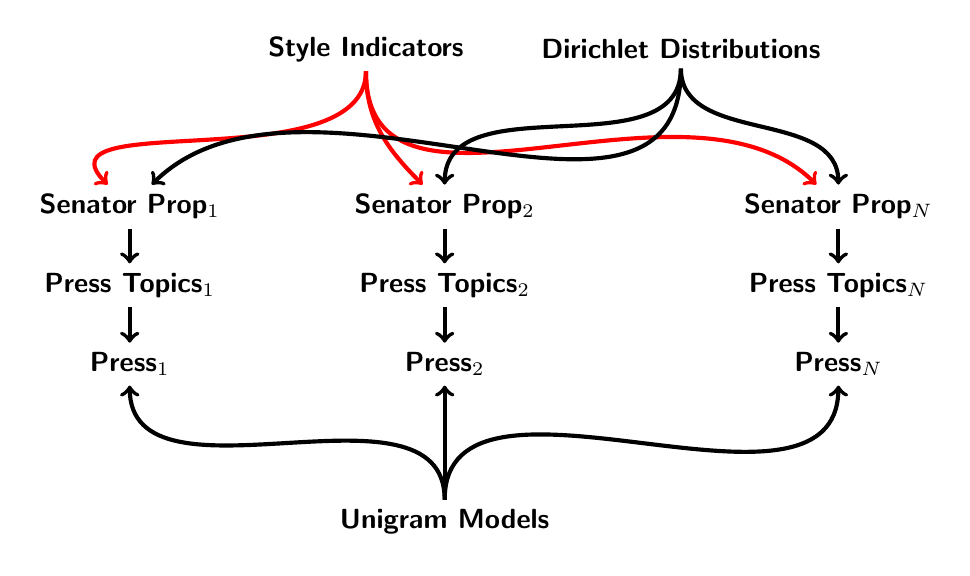
\begin{tikzpicture}

\node (col1) at (-2, 10) [] {\textbf{Style Indicators} } ; 
\node (col) at (2, 10) [] {\textbf{Dirichlet Distributions} }  ; 




\node (doc1) at (-5, 8) [] {\textbf{Senator Prop}$_{1}$} ; 
\node (doc2) at (-1, 8) [] {\textbf{Senator Prop}$_{2}$} ; 
\node (dots) at ( 2, 8) [] {$\hdots$} ; 
\node (docN) at (4, 8) [] {\textbf{Senator Prop}$_{N}$} ; 


\draw[->, line width=1.5pt, red] (col1) to [out=270, in = 135] (doc1); 
\draw[->, line width=1.5pt, red] (col1) to [out=270, in = 135] (doc2); 
\draw[->, line width=1.5pt, red] (col1) to [out=270, in = 135] (docN); 



\draw[->, line width=1.5pt] (col) to [out=270, in = 45] (doc1); 
\draw[->, line width=1.5pt] (col) to [out=270, in = 90] (doc2); 
\draw[->, line width=1.5pt] (col) to [out=270, in = 90] (docN); 





\node (word11) at (-5, 7) [] {\textbf{Press Topics}$_{1}$} ; 
\node (word22) at (-1, 7) [] {\textbf{Press Topics}$_{2}$} ; 
\node (wordnn) at (4, 7) [] {\textbf{Press Topics}$_{N}$ } ; 

\draw[->, line width=1.5pt] (doc1) to [out=270, in=90] (word11) ; 
\draw[->, line width=1.5pt] (doc2) to [out=270, in=90] (word22) ; 
\draw[->, line width=1.5pt] (docN) to [out=270, in=90] (wordnn) ; 



\node (wordaa) at (-5, 6) [] {\textbf{Press}$_{1}$} ; 
\node (wordbb) at (-1, 6) [] {\textbf{Press}$_{2}$} ; 
\node (wordcc) at (4, 6) [] {\textbf{Press}$_{N}$ } ; 


\draw[->, line width = 1.5pt] (word11) to [out = 270, in = 90] (wordaa); 
\draw[->, line width = 1.5pt] (word22) to [out = 270, in = 90] (wordbb); 
\draw[->, line width = 1.5pt] (wordnn) to [out = 270, in = 90] (wordcc); 

\node (topics) at (-1, 4) [] {$\textbf{Unigram Models}$} ; 



\draw[->, line width = 1.5pt] (topics) to [out = 90, in = 270] (wordaa); 
\draw[->, line width = 1.5pt] (topics) to [out = 90, in = 270] (wordbb); 
\draw[->, line width = 1.5pt] (topics) to [out = 90, in = 270] (wordcc); 



\end{tikzpicture}



\end{frame}



\begin{frame}

Posterior: \tiny
\begin{eqnarray}
p(\boldsymbol{\alpha}, \boldsymbol{\beta}, \boldsymbol{\theta},
\boldsymbol{\sigma}, \boldsymbol{\pi},
\boldsymbol{\tau}|\boldsymbol{X}) & \propto &
\prod_{k=1}^{K}\prod_{s=1}^{S} \frac{\exp( -
\frac{\alpha_{ks}}{1/4})}{1/4} \times \frac{\Gamma(\sum_{w=1}^{W}
\lambda_w) }{\prod_{w=1}^{W} \Gamma(\lambda_w) } \prod_{w=1}^{W}
\theta_{k,w}^{\lambda_w - 1}
\times \nonumber \\
& & \prod_{i=1}^{N} \prod_{t=2005}^{2007} \prod_{s=1}^{S} \left[
\beta_s \frac{\Gamma(\sum_{k=1}^{K} \alpha_{ks})}{\prod_{k=1}^{K}
\Gamma(\alpha_{ks} )} \prod_{k=1}^{K} \pi_{itk}^{\alpha_{ks}-1}
\prod_{j=1}^{D_{it} }\prod_{k=1}^{K} \left[ \pi_{itk}
\prod_{w=1}^{W} \theta_{kw} ^{x_{ijtw} }
 \right]^{\tau_{ijtk}} \right]^{\sigma_{its}} \nonumber
\end{eqnarray}

\pause 


\normalsize
\begin{itemize}
\invisible<1>{\item[1)] Estimate with Variational Approximation} \pause 
\invisible<1-2>{\item[2)] Determining number of clusters at top? (Grimmer, Shorey, Wallach, and Zlotnick, In Progress)} \pause
\begin{itemize}
\invisible<1-3>{\item[-] Non-parametric model$\leadsto$ statistical selection} \pause
\invisible<1-4>{\item[-] Experiments/Coding Exercises to assess} 
\end{itemize} 

\end{itemize}


\end{frame}


\begin{frame}


\only<1>{\scalebox{0.35}{\includegraphics{ShelbyPress.pdf}}}
\only<2>{\scalebox{0.35}{\includegraphics{SessionsPress.pdf}}} 




\end{frame}


\begin{frame}
\frametitle{Notions of validity: From Quinn, Monroe, et al (2010) } 

\begin{enumerate}
\item[-] \alert{Semantic Validity:} All categories are coherent and meaningful
\item[-] \alert{Convergent Construct Validity:} Measures concur with existing measures in critical details.
\item[-]  \alert{Discriminant Construct Validity}: Measures differ from existing measures in productive ways.  
\item[-] \alert{Predictive Measure:} Measures from the model corresponds to external events in expected ways.
\item[-] \alert{Hypothesis Validity:} Measures generated from the model can be used to test substantive hypotheses. 
\end{enumerate}

To establish utility of new measures, demonstrate variety of \alert{validations}\\
\alert{None of these validations are performed using a canned statistic}\\
\alert{All}: require substantive knowledge on areas (and what we expect!) [

\end{frame}


\begin{frame}
\frametitle{Home Style Measures, Semantic Validity} 


\alert{Must}: Demonstrate to reader that topics are coherent and semantically meaningful

\begin{tabular}{lll}
\hline\hline
Description & Stems & \% \\
\hline
Honorary& honor,prayer,rememb,fund,tribut& 5.0\\
Transp. Grants& airport,transport,announc,urban,hud&4.8\\
Iraq& iraq,iraqi,troop,war,sectarian& 4.7\\
DHS Policy& homeland,port,terrorist,dh,fema&4.1\\
Judicial Nom.& judg,court,suprem,nomin,nomine&3.8\\
Fire Dept. Grant& firefight,homeland,afgp,award,equip&3.7\\
\hline
\end{tabular}

How: \alert{examples} in text are also useful.  


\end{frame}


\begin{frame}
\frametitle{Home Style Measures, Convergent Validity} 

\only<1-3>{\alert{Over time variation} }
\only<4>{\alert{Supervised/Unsupervised Convergence} } 
\only<1>{\scalebox{0.4}{\includegraphics{ImmigrationPlot.pdf}}}
\only<2>{\scalebox{0.4}{\includegraphics{IraqWarPlot.pdf}}}
%\only<3>{\scalebox{0.4}{\includegraphics{Worker5.pdf}}}
\only<3>{\scalebox{0.4}{\includegraphics{HonorPlot.pdf}}} 

\only<4>{\scalebox{0.3}{\includegraphics{SupervisedUnsupervised.pdf}}}
\only<5>{\scalebox{0.3}{\includegraphics{ConvValid.pdf}}}

\end{frame}


\begin{frame}
\frametitle{Discriminant Construct Validity} 

\scalebox{0.45}{\includegraphics{IdealAttn.pdf} } 


\end{frame}



\begin{frame}
\frametitle{Predictive Validity} 


\scalebox{0.4}{\includegraphics{CompareLeaders.pdf} } 


\end{frame}


\begin{frame}
\frametitle{Hypothesis Validity}


\scalebox{0.28}{\includegraphics{PrioritiesPlotLabel.pdf}}

\begin{columns}[]
\invisible<1>{\column{0.25\textwidth}
\textcolor{blue}{Senate}\\
\textcolor{blue}{Statesperson}
\begin{itemize}
\item[-] \textcolor{blue}{Iraq War}
\item[-] \textcolor{blue}{Intelligence}
\item[-] \textcolor{blue}{Intl. Relations}
\item[-] \textcolor{blue}{Budget}
\end{itemize}}

\invisible<1-2>{\column{0.25\textwidth}
\textcolor{darkgreen}{Domestic}\\
\textcolor{darkgreen}{Policy}
\begin{itemize}
\item[-] \textcolor{darkgreen}{Environment}
\item[-] \textcolor{darkgreen}{Gas prices}
\item[-] \textcolor{darkgreen}{DHS}
\item[-] \textcolor{darkgreen}{Consumer Safety}
\end{itemize}}

\invisible<1-3>{\column{0.25\textwidth} \textcolor{brown}{Pork \&
Policy}
\begin{itemize}
\item[-] \textcolor{brown}{WRDA grants}
\item[-] \textcolor{brown}{Farming}
\item[-] \textcolor{brown}{Health Care}
\item[-] \textcolor{brown}{Education Policy}
\end{itemize}}

\invisible<1-4>{\column{0.25\textwidth}
\textcolor{red}{Appropriators}
\begin{itemize}
\item[-] \textcolor{red}{Fire Grants}
\item[-] \textcolor{red}{Airport Grants}
\item[-] \textcolor{red}{University Money}
\item[-] \textcolor{red}{Police Grants}
\end{itemize}}


\end{columns}

\pause\pause\pause\pause
\end{frame}

\begin{frame}
\frametitle{Hypothesis Validity}


Why do senators adopt different styles?\\
\alert{District Fit} 

\scalebox{0.4}{\includegraphics{FinalAvoidance.pdf}}



\end{frame}


\begin{frame}
\frametitle{What are the right number of topics?}

\pause 

\begin{itemize}
\invisible<1>{\item[-] Number of topics$\leadsto$ depends on task at hand}
\invisible<1-2>{\item[-] Coarse$\leadsto$ broad comparisons, lose distinctions}
\invisible<1-3>{\item[-] Granular$\leadsto$ specific insights, lose broader picture}
\invisible<1-4>{\item[-] \alert{Hierarchy of topics}$\leadsto$ Pachinko Allocation, Hierarchies of von-Mises Fisher Distributions}
\end{itemize}

\invisible<1-5>{Blaydes, Grimmer, and McQueen [In Progress]$\leadsto$ estimate nested topics to explore the \alert{Mirros for Princes}}


\pause \pause \pause \pause 



\end{frame}




\begin{frame}
\frametitle{The Mirrors Genre}


26 Christian mirrors \pause 
\begin{itemize}
\invisible<1>{\item[-] The Prince (1513 CE)} \pause 
\invisible<1-2>{\item[-] Advice to Justinian (527 CE)} \pause 
\invisible<1-3>{\item[-] The Adventures of Telemachus (1699 CE)} \pause 
\end{itemize}


\invisible<1-4>{21 Islamic texts} \pause 
\begin{itemize}
\invisible<1-5>{\item[-] Advice on the Art of Governance (1612 CE)} \pause
\invisible<1-6>{\item[-] Kalila wa Dimna (748 CE)} \pause
\invisible<1-7>{\item[-] The Sultan's Register of Laws (1632-1633 CE)} \pause 
\end{itemize}



\invisible<1-8>{Work with translations}\pause\invisible<1-9>{$\leadsto$ little evidence of selection} \pause 
\begin{itemize}
\invisible<1-10>{\item[-] Collect data on collection of 98 (51 Christian, 47 Islamic, some not translated)} \pause 
\invisible<1-11>{\item[-] No difference on Year/Region} 
\end{itemize}


\end{frame}




\begin{frame}
\frametitle{Preprocessing Texts}

47 books \invisible<1>{$\leadsto$ Each divided into paragraphs} \\
\invisible<1-2>{Create feature space} 
\begin{itemize}
\invisible<1-3>{\item[-] Bag of words, stem, discard punctuation, stop words}
\invisible<1-4>{\item[-] Translate words left in Arabic (\alert{allah}) and discard proper nouns}
\invisible<1-5>{\item[-] Identified synonyms} 
\begin{itemize}
\invisible<1-6>{\item[-] \alert{almighty}, \alert{god}}
\invisible<1-7>{\item[-] \alert{monarch}, \alert{prince}, \alert{king}, \alert{ruler}}
\invisible<1-8>{\item[-] \alert{Lord} $\neq$ \alert{lord} }
\end{itemize}
\end{itemize}

\invisible<1-9>{Result: short segment $j$ in book $i$ is a count vector} 
\begin{eqnarray}
\invisible<1-10>{\textbf{x}_{ij} & = & (x_{ij1}, x_{ij2}, \hdots, x_{ij2124}) \nonumber}
\end{eqnarray}

\invisible<1-11>{We work with a normalized version of the documents, }
\begin{eqnarray}
\invisible<1-12>{\textbf{x}^{*}_{ij} & = & \frac{\textbf{x}_{ij}}{\sqrt{\textbf{x}^{'}_{ij}\textbf{x}_{ij}} } \nonumber}
\end{eqnarray}



\pause \pause \pause \pause \pause \pause \pause \pause \pause \pause \pause \pause 


\end{frame}




\begin{frame}
\frametitle{Measuring Themes in the Mirrors}

\only<1-3>{Model built around two hierarchies: 
\begin{itemize}
\invisible<1>{\item[1)] Books $\leadsto$ paragraphs (Blei, Ng, Jordan 2003; Wallach, 2008; Quinn et al 2010; Grimmer 2010; Roberts et al 2014)}
\invisible<1-2>{\item[2)] Coarse topics $\leadsto$ granular topics (Li and McCallum 2006; Gopal and Yang 2014)}
\end{itemize}
}


\only<4->{
Estimate \alert{four} quantities of interest
\begin{itemize}
\invisible<1-4>{\item[1)] Granular topics (60)} 
\invisible<1-5>{\item[2)] Coarse (broad) topics (3)} 
\begin{itemize}
\invisible<1-6>{\item[-] Each granular topic classified into one coarse topic } 
\end{itemize}
\invisible<1-7>{\item[3)] Each book $i'$s  $\textbf{themes}_{i}}$ 
\invisible<1-8>{\item[4)] Each short segment's granular (and coarse) topic } 
\end{itemize}




\begin{eqnarray}
\invisible<1-7, 9->{\textbf{themes}_{i} & = & (\text{theme}_{i1}, \text{theme}_{i2}, \hdots, \text{theme}_{i60} ) \nonumber }
\end{eqnarray}

}



\pause \pause \pause \pause \pause \pause \pause \pause 
\end{frame}

\begin{frame}
\frametitle{A Hierarchy of Topics}


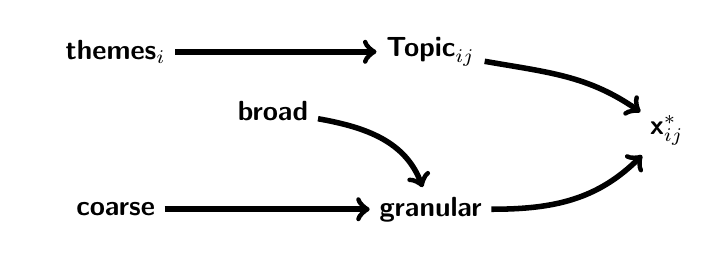
\begin{tikzpicture}

\node (Dummy) at (-9,8) [] {} ; 
\node (theme1) at (-8, 9) [] {$\textbf{themes}_{i} $} ; 
\invisible<1>{\node (draws) at (-4, 9) [] {$\textbf{Topic}_{ij}$};}
\invisible<1>{\draw[->, line width = 2pt] (theme1) to [out = 0, in = 180] (draws);}

\invisible<1-2>{\node (document) at (-1, 8) [] {$\textbf{x}^{*}_{ij}$ }; }
\invisible<1-2>{\draw[->, line width = 2pt] (draws) to [out = 350, in  = 145] (document); }


\invisible<1-2>{\node (topics)   at (-4, 7) [] {$\textbf{granular}$}; } 

\invisible<1-2>{\draw[->, line width = 2pt] (topics) to [out = 0, in = 225] (document) ; }

\invisible<1-3>{\node (topic_sig) at (-6, 8.25) [] {$\textbf{broad}$} ; }

\invisible<1-3>{\draw[->, line width = 2pt] (topic_sig) to [out = 350, in = 110] (topics) ; }

\invisible<1-3>{\node (coarse)    at (-8, 7) [] {$\textbf{coarse}$}; }

\invisible<1-3>{\draw[->, line width = 2pt] (coarse) to [out = 0, in= 180] (topics) ; }

\end{tikzpicture}


\begin{eqnarray}
\invisible<1>{\textbf{Topic}_{ij} & \sim & \text{Multinomial}(1, \textbf{themes}_{i}) \nonumber }\\
\invisible<1-2>{\textbf{x}^{*}_{ij} | \text{Topic}_{ijk} =  1 & \sim & \text{vMF} (\kappa, \textbf{granular}_{k} ) \nonumber }\\
\invisible<1-3>{\textbf{broad}_{k} & \sim & \text{Multinomial}(1, \textbf{Broad Theme Prior}) \nonumber }\\
\invisible<1-3>{\textbf{granular}_{k} | \text{broad}_{km} = 1 & \sim & \text{vMF}(\kappa, \textbf{coarse}_{m}) \nonumber }
\end{eqnarray}

\invisible<1-4>{Estimate model with Variational Approximation}\\
\invisible<1-5>{Model selection: automatic model fit, qualitative evaluation}

\pause \pause \pause \pause \pause 




%%draws theme
%%then draws content from a topic specific distribution
%%our model classifies each of those granular themes into coarse themes



\end{frame}





\begin{frame}
\frametitle{Interpreting Unsupervised Models}

Two approaches to labeling output \pause  
\begin{itemize}
\invisible<1>{\item[1)] \alert{Computational}: identify discriminating words }\pause 
\invisible<1-2>{\item[2)] \alert{Manual}: Segments classified to coarse, granular topics.  Read, discuss, and label} \pause 
\end{itemize}

\invisible<1-3>{Unsupervised models \alert{structure} and \alert{guide} our reading}




\end{frame}



\begin{frame}
\frametitle{Art of Rulership}


Practices and ideals of political rule

\vspace{0.5in}
\begin{tabular}{l}
\invisible<1>{king}\invisible<1-2>{,princ}\invisible<1-3>{,citi}\invisible<1-4>{,great,place,work,emperor,enemi,armi,letter} \\
\end{tabular}

\vspace{0.5in}
 \invisible<1-5>{36.5\% of paragraphs } 

\pause \pause \pause \pause \pause 


\end{frame}

\begin{frame}

\begin{center}
\scalebox{0.45}{\includegraphics{Hist_Super1_p.pdf}}
\end{center}

\end{frame}


\begin{frame}

\begin{center}
\scalebox{0.45}{\includegraphics{Super1.pdf}}
\end{center}


\end{frame}


\begin{frame}
\frametitle{Religion and Virtue}


Connection between religion, virtue, justice and political rule \pause 

\vspace{0.5in}
\begin{tabular}{l}
\invisible<1>{almighti,good,virtu,power,ruler,justic,prayer,rule,prophet,mena \\}
\end{tabular}

\pause 
\vspace{0.5in}

\invisible<1-2>{32.2\% of pargraphs} 

\end{frame}


\begin{frame}

\begin{center}
\scalebox{0.45}{\includegraphics{Hist_Super2_p.pdf}}
\end{center}

\end{frame}



\begin{frame}

\begin{center}
\scalebox{0.45}{\includegraphics{Super2.pdf}}
\end{center}

\end{frame}






\begin{frame}
\frametitle{Inner Life of the Ruler}

Personal relationships, care for and practices of the self, and ultimate fate of the soul \pause 

\vspace{0.5in}

\begin{tabular}{ll}
\invisible<1>{man,land,woman,know,bodi,eye,ladi,love,faculti,old} \pause 
\end{tabular}

\vspace{0.5in}

\invisible<1-2>{31.2\% of paragraphs} 

\end{frame}



\begin{frame}


\begin{center}
\scalebox{0.45}{\includegraphics{Hist_Super3_p.pdf}}
\end{center}

\end{frame}




\begin{frame}

\begin{center}
\scalebox{0.45}{\includegraphics{Super3.pdf}}
\end{center}

\end{frame}



\begin{frame}
\frametitle{Granular: Best Practices for Ruling}


\begin{tabular}{l}
\hline
king,princ,citi,great,place,work,emperor,enemi,armi,letter \\
\hline
\alert{king,kingdom,royal,minist,reign,father,court,majesti,presenc,war}
\end{tabular}

\vspace{0.5in}

6.2\% of paragraphs

\end{frame}



\begin{frame}

\begin{center}
\scalebox{0.45}{\includegraphics{1point1.pdf}}
\end{center}

\end{frame}


\begin{frame}
\frametitle{Granular: Characteristics that distinguish Just Ruler from Tyrant}


\begin{tabular}{l}
\hline
king,princ,citi,great,place,work,emperor,enemi,armi,letter \\
\hline
king,kingdom,royal,minist,reign,father,court,majesti,presenc,war\\
\alert{princ,good,peopl,christian,tyranni,war,mind,ought,state,public}\\
\end{tabular}

\vspace{0.5in}

3.1\% of paragraphs

\end{frame}


\begin{frame}

\begin{center}
\scalebox{0.45}{\includegraphics{1point2.pdf}}
\end{center}

\end{frame}


\begin{frame}
\frametitle{Granular: Religious Virtues and Political Ideals}


\begin{tabular}{l}
\hline
almighti,good,virtu,power,ruler,justic,prayer,rule,prophet,mena\\
\hline 
\alert{almighti,bless,grant,peac,messeng,prophet,merci,holi,command,grace}
\end{tabular}

\vspace{0.5in}

6.9\% of paragraphs


\end{frame}



\begin{frame}

\begin{center}
\scalebox{0.45}{\includegraphics{2point1.pdf}}
\end{center}

\end{frame}


\begin{frame}
\frametitle{Structural Topic Models}

\begin{itemize}
\item[-] Encode observed and unobserved meta data
\item[-] ?Improve substantive inferences
\end{itemize}

Next week:
\begin{itemize}
\item[1)] Hanna Wallach on canonical topic models
\item[2)] Introduction to supervised learning
\end{itemize}

Work on your problem sets!

\end{frame}


\begin{frame}

Appendix: Inference for both Models


\end{frame}




\begin{frame}
\frametitle{Inference}

Invariance in posterior makes it difficult (impossible) to
approximate with sampling based methods (relabeling, aliasing problem).  \\

Deterministic alternative: variational approximations.  \\

Intuition: approximate posterior with simpler (still very general)
approximating distribution. \\

Make approximation as ``close" as possible\\

\end{frame}

\begin{frame}
Approximate posterior with:

\scriptsize
\begin{eqnarray}
q(\boldsymbol{\alpha}, \boldsymbol{\beta}, \boldsymbol{\theta},
\boldsymbol{\sigma}, \boldsymbol{\pi}, \boldsymbol{\tau}) & = &
q(\boldsymbol{\alpha})q(\boldsymbol{\beta})q( \boldsymbol{\theta})q(\boldsymbol{\sigma})q(\boldsymbol{\pi})q(\boldsymbol{\tau}) \nonumber \\
& = & q(\boldsymbol{\beta} ) \prod_{k=1}^{K}
q(\boldsymbol{\theta})_{k} \prod_{i=1}^{n}
\prod_{t=2005}^{2007}\left[ q(\boldsymbol{\sigma})_{it}
q(\boldsymbol{\pi})_{it}
 \prod_{j=1}^{J} q(\boldsymbol{\tau})_{ijt} \right] \prod_{s=1}^{S} q(\boldsymbol{\alpha})_{s}
 \nonumber
\end{eqnarray}

\end{frame}


\begin{frame}
\frametitle{Variational Approximation} Optimization goal:
\begin{itemize}
\item[-] Minimize the Kullback-Leibler divergence
between approximating distribution $q$ and true posterior $p$
\begin{itemize}
\item[-] KL-divergence is a functional: takes
\alert{functions} as an input, returns a positive scalar
\item[-] Measures ``divergence" between two
measures
\end{itemize}
\item[-] Use calculus of variations and theory from
exponential models to derive iterative algorithm
\item[-] See ``An Introduce to Bayesian Inference via Variational
Approximations" for extended introduction (Grimmer, 2011)
\end{itemize}
\end{frame}






\begin{frame}
\frametitle{Minimize KL-divergence by Maximizing a Lower Bound}

\scriptsize
\begin{eqnarray}
\log p(\boldsymbol{Y}) & = & \log
\sum_{\boldsymbol{\sigma}}\sum_{\boldsymbol{\tau}} \iiiint
p(\boldsymbol{\alpha}, \boldsymbol{\beta}, \boldsymbol{\theta},
\boldsymbol{\sigma}, \boldsymbol{\pi},
\boldsymbol{\tau}|\boldsymbol{Y}) d\boldsymbol{\theta}
d\boldsymbol{\alpha}d\boldsymbol{\beta}d\boldsymbol{\pi} \nonumber
\end{eqnarray}



\begin{eqnarray}
\log p(\boldsymbol{Y}) & = & \log
\sum_{\boldsymbol{\sigma}}\sum_{\boldsymbol{\tau}} \iiiint
p(\boldsymbol{\alpha}, \boldsymbol{\beta}, \boldsymbol{\theta},
\boldsymbol{\sigma}, \boldsymbol{\pi},
\boldsymbol{\tau}|\boldsymbol{Y}) \frac{q(\boldsymbol{\alpha},
\boldsymbol{\beta}, \boldsymbol{\theta}, \boldsymbol{\sigma},
\boldsymbol{\pi}, \boldsymbol{\tau})}{q(\boldsymbol{\alpha},
\boldsymbol{\beta}, \boldsymbol{\theta}, \boldsymbol{\sigma},
\boldsymbol{\pi}, \boldsymbol{\tau})}d\boldsymbol{\theta}
d\boldsymbol{\alpha}d\boldsymbol{\beta}d\boldsymbol{\pi} \nonumber
\end{eqnarray}


\begin{eqnarray}
\log p(\boldsymbol{Y}) & \geq &
\underbrace{\sum_{\boldsymbol{\sigma}}\sum_{\boldsymbol{\tau}}
\iiiint q(\boldsymbol{\alpha}, \boldsymbol{\beta},
\boldsymbol{\theta}, \boldsymbol{\sigma}, \boldsymbol{\pi},
\boldsymbol{\tau}) \log\frac{p(\boldsymbol{\alpha},
\boldsymbol{\beta}, \boldsymbol{\theta}, \boldsymbol{\sigma},
\boldsymbol{\pi},
\boldsymbol{\tau}|\boldsymbol{Y})}{q(\boldsymbol{\alpha},
\boldsymbol{\beta}, \boldsymbol{\theta}, \boldsymbol{\sigma},
\boldsymbol{\pi}, \boldsymbol{\tau})}d\boldsymbol{\theta}
d\boldsymbol{\alpha}d\boldsymbol{\beta}d\boldsymbol{\pi}}_{\mathcal{L}(q)
}. \nonumber
\end{eqnarray}

\end{frame}


\begin{frame}
\frametitle{Minimize KL-divergence by Maximizing a Lower Bound}

\begin{eqnarray}
\log p(\boldsymbol{Y}) & =& \mathcal{L}(q) + \text{KL}(q||p)
\nonumber
 \\ \pause
\invisible<1>{\underbrace{\log p(\boldsymbol{Y})}_{\text{fixed
number}} & =& \mathcal{L}(q) +
\underbrace{\text{KL}(q||p)}_{\text{Positive}} \nonumber}
\end{eqnarray}
\pause  \invisible<1-2>{If $\mathcal{L}(q)$ get bigger,
$\text{KL}(q||p)$
get smaller. $\Rightarrow$} \pause \\
\invisible<1-3>{If $\mathcal{L}(q)$ is at a maximum
$\text{KL}(q||p)$ is at a minimum (duals).}
\end{frame}


\begin{frame}
\frametitle{Maximizing $\mathcal{L}(q)$}

Goal: choose $q$ to maximize $\mathcal{L}(q)$.  \\

\begin{eqnarray}
q(\boldsymbol{\alpha})^{\text{old}},
q(\boldsymbol{\beta})^{\text{old}}, q(
\boldsymbol{\theta})^{\text{old}},
q(\boldsymbol{\sigma})^{\text{old}},
q(\boldsymbol{\pi})^{\text{old}}, q(\boldsymbol{\tau})^{\text{old}}.
\nonumber
\end{eqnarray}

Iterative Algorithm:  \\
\footnotesize Choose, $q(\boldsymbol{\pi})^{\text{new}}$ to max
$\mathcal{L}(q)$--holding
$q(\boldsymbol{\theta})^{\text{old}},q(\boldsymbol{\tau})^{\text{old}},q(\boldsymbol{\alpha})^{\text{old}},
q(\boldsymbol{\beta})^{\text{old}},q(\boldsymbol{\sigma})^{\text{old}}$
constant. \\
Choose, $q(\boldsymbol{\theta})^{\text{new}}$ to max
$\mathcal{L}(q)$--holding
$q(\boldsymbol{\pi})^{\text{new}},q(\boldsymbol{\tau})^{\text{old}},q(\boldsymbol{\alpha})^{\text{old}},
q(\boldsymbol{\beta})^{\text{old}},q(\boldsymbol{\sigma})^{\text{old}}$
constant. \\
Choose, $q(\boldsymbol{\tau})^{\text{new}}$ to max
$\mathcal{L}(q)$--holding
$q(\boldsymbol{\theta})^{\text{new}},q(\boldsymbol{\pi})^{\text{new}},q(\boldsymbol{\alpha})^{\text{old}},
q(\boldsymbol{\beta})^{\text{old}},q(\boldsymbol{\sigma})^{\text{old}}$
constant. \\
Choose, $q(\boldsymbol{\alpha})^{\text{new}}$ to max
$\mathcal{L}(q)$--holding
$q(\boldsymbol{\theta})^{\text{new}},q(\boldsymbol{\tau})^{\text{new}},q(\boldsymbol{\pi})^{\text{new}},
q(\boldsymbol{\beta})^{\text{old}},q(\boldsymbol{\sigma})^{\text{old}}$
constant. \\
Choose, $q(\boldsymbol{\beta})^{\text{new}}$ to max
$\mathcal{L}(q)$--holding
$q(\boldsymbol{\theta})^{\text{new}},q(\boldsymbol{\tau})^{\text{new}},q(\boldsymbol{\pi})^{\text{new}},
q(\boldsymbol{\alpha})^{\text{new}},q(\boldsymbol{\sigma})^{\text{old}}$
constant. \\
Choose, $q(\boldsymbol{\sigma})^{\text{new}}$ to max
$\mathcal{L}(q)$--holding
$q(\boldsymbol{\theta})^{\text{new}},q(\boldsymbol{\tau})^{\text{new}},q(\boldsymbol{\pi})^{\text{new}},
q(\boldsymbol{\alpha})^{\text{new}},q(\boldsymbol{\beta})^{\text{new}}$
constant.
\end{frame}

\begin{frame}
\frametitle{Example for $q(\boldsymbol{\pi})^{\text{new}}$} \tiny
\begin{eqnarray}
\mathcal{L}(q) & =& \int q(\boldsymbol{\pi})^{\text{new}}
\underbrace{\left\{ \sum_{\boldsymbol{\sigma}}
\sum_{\boldsymbol{\tau}} \iiint \log p(\boldsymbol{Y},
\boldsymbol{\pi}, \boldsymbol{\alpha}, \boldsymbol{\theta},
\boldsymbol{\tau})
q(\boldsymbol{\sigma})^{\text{old}}q(\boldsymbol{\tau})^{\text{old}}q(\boldsymbol{\theta})^{\text{old}}q(\boldsymbol{\alpha})^{\text{old}}q(\boldsymbol{\beta})^{\text{old}}
d\boldsymbol{\theta} d\boldsymbol{\alpha}
d\boldsymbol{\beta}\right\}}_{\text{E}_{\boldsymbol{\alpha},
\boldsymbol{\tau}, \boldsymbol{\theta}, \boldsymbol{\sigma},
\boldsymbol{\beta} }[\log p(\boldsymbol{Y}, \boldsymbol{\pi},
\boldsymbol{\alpha},
\boldsymbol{\theta}, \boldsymbol{\tau}, \boldsymbol{\beta}, \boldsymbol{\sigma})]}d\boldsymbol{\pi} \nonumber \\
&&- q(\boldsymbol{\pi})^{\text{new}}\log
q(\boldsymbol{\pi})^{\text{new}} + \text{constants} \nonumber
\end{eqnarray}
\normalsize Define
\begin{eqnarray}
\log \tilde{p}(\boldsymbol{\pi}) & = &
\text{E}_{\boldsymbol{\alpha}, \boldsymbol{\tau},
\boldsymbol{\theta}, \boldsymbol{\sigma}, \boldsymbol{\beta} }[\log
p(\boldsymbol{Y}, \boldsymbol{\pi}, \boldsymbol{\alpha},
\boldsymbol{\theta}, \boldsymbol{\tau}, \boldsymbol{\beta},
\boldsymbol{\sigma})] + \text{constants} \nonumber
\end{eqnarray}


\end{frame}

\begin{frame}
\frametitle{Example for $q(\boldsymbol{\pi})^{\text{new}}$}
Substituting $\log \tilde{p}(\boldsymbol{\pi})$,
\begin{eqnarray}
& = & \int q(\boldsymbol{\pi})^{\text{new}} \log
\left(\frac{\tilde{p}(\boldsymbol{\pi})}{q(\boldsymbol{\pi})^{\text{new}}}
\right)d\boldsymbol{\pi} \nonumber \\
& = & -
\text{KL}(q(\boldsymbol{\pi})^{\text{new}}||\tilde{p}(\boldsymbol{\pi})
) \nonumber
\end{eqnarray}
$\Rightarrow$ At a maximum when $q(\boldsymbol{\pi})^{\text{new}}
=\tilde{p}(\boldsymbol{\pi}) $.  \\
Equivalently,
\begin{eqnarray}
\log q(\boldsymbol{\pi})^{\text{new}} & = & \log
\tilde{p}(\boldsymbol{\pi}) \nonumber \\
& = & \text{E}_{\boldsymbol{\alpha}, \boldsymbol{\tau},
\boldsymbol{\theta}, \boldsymbol{\sigma}, \boldsymbol{\beta} }[\log
p(\boldsymbol{Y}, \boldsymbol{\pi}, \boldsymbol{\alpha},
\boldsymbol{\theta}, \boldsymbol{\tau}, \boldsymbol{\beta},
\boldsymbol{\sigma})] + \text{constants}\nonumber
\end{eqnarray}
Or,
\begin{eqnarray}
q(\boldsymbol{\pi})^{\text{new}} & = &
\frac{\exp(\text{E}_{\boldsymbol{\alpha}, \boldsymbol{\tau},
\boldsymbol{\theta}, \boldsymbol{\sigma}, \boldsymbol{\beta} }[\log
p(\boldsymbol{Y}, \boldsymbol{\pi}, \boldsymbol{\alpha},
\boldsymbol{\theta}, \boldsymbol{\tau}, \boldsymbol{\beta},
\boldsymbol{\sigma})])}{\int \exp(\text{E}_{\boldsymbol{\alpha},
\boldsymbol{\tau}, \boldsymbol{\theta}, \boldsymbol{\sigma},
\boldsymbol{\beta} }[\log p(\boldsymbol{Y}, \boldsymbol{\pi},
\boldsymbol{\alpha}, \boldsymbol{\theta}, \boldsymbol{\tau},
\boldsymbol{\beta}, \boldsymbol{\sigma})])d\boldsymbol{\pi}}
\nonumber
\end{eqnarray}

\end{frame}


\begin{frame}
To maximize $\mathcal{L}(q)$ we use the following iterative
algorithm \scriptsize
\begin{eqnarray}
q(\boldsymbol{\sigma})^{\text{new}} & \propto &
\exp\left(\text{E}_{\boldsymbol{\tau}, \boldsymbol{\theta},
\boldsymbol{\alpha}, \boldsymbol{\beta}, \boldsymbol{\pi} }[\log
p(\boldsymbol{\alpha}, \boldsymbol{\beta}, \boldsymbol{\theta},
\boldsymbol{\sigma}, \boldsymbol{\pi}, \boldsymbol{\tau},
\boldsymbol{Y}) ] \right) \nonumber \\
q(\boldsymbol{\tau})^{\text{new}} & \propto &
\exp\left(\text{E}_{\boldsymbol{\sigma}, \boldsymbol{\theta},
\boldsymbol{\alpha}, \boldsymbol{\beta}, \boldsymbol{\pi} }[\log
p(\boldsymbol{\alpha}, \boldsymbol{\beta}, \boldsymbol{\theta},
\boldsymbol{\sigma}, \boldsymbol{\pi}, \boldsymbol{\tau},
\boldsymbol{Y}) ] \right) \nonumber \\
q(\boldsymbol{\theta})^{\text{new}} & \propto &
\exp\left(\text{E}_{\boldsymbol{\sigma}, \boldsymbol{\tau},
\boldsymbol{\alpha}, \boldsymbol{\beta}, \boldsymbol{\pi} }[\log
p(\boldsymbol{\alpha}, \boldsymbol{\beta}, \boldsymbol{\theta},
\boldsymbol{\sigma}, \boldsymbol{\pi}, \boldsymbol{\tau},
\boldsymbol{Y}) ] \right) \nonumber \\
q(\boldsymbol{\alpha})^{\text{new}} & \propto &
\exp\left(\text{E}_{\boldsymbol{\sigma}, \boldsymbol{\tau},
\boldsymbol{\theta}, \boldsymbol{\beta}, \boldsymbol{\pi} }[\log
p(\boldsymbol{\alpha}, \boldsymbol{\beta}, \boldsymbol{\theta},
\boldsymbol{\sigma}, \boldsymbol{\pi}, \boldsymbol{\tau},
\boldsymbol{Y}) ] \right) \nonumber \\
q(\boldsymbol{\beta})^{\text{new}} & \propto &
\exp\left(\text{E}_{\boldsymbol{\sigma}, \boldsymbol{\tau},
\boldsymbol{\theta}, \boldsymbol{\alpha}, \boldsymbol{\pi} }[\log
p(\boldsymbol{\alpha}, \boldsymbol{\beta}, \boldsymbol{\theta},
\boldsymbol{\sigma}, \boldsymbol{\pi}, \boldsymbol{\tau},
\boldsymbol{Y}) ] \right) \nonumber \\
q(\boldsymbol{\pi})^{\text{new}} & \propto &
\exp\left(\text{E}_{\boldsymbol{\sigma}, \boldsymbol{\tau},
\boldsymbol{\theta}, \boldsymbol{\alpha}, \boldsymbol{\beta} }[\log
p(\boldsymbol{\alpha}, \boldsymbol{\beta}, \boldsymbol{\theta},
\boldsymbol{\sigma}, \boldsymbol{\pi}, \boldsymbol{\tau},
\boldsymbol{Y}) ] \right) \nonumber
\end{eqnarray}
\end{frame}

\begin{frame}
\frametitle{Update for $q(\boldsymbol{\sigma})_{it}$}
$q(\boldsymbol{\sigma})_{it}$ is a Multinomial$(1,
\boldsymbol{c}_{it})$ distribution, with typical parameter $c_{its}$

\scriptsize

\begin{eqnarray}
\boldsymbol{c}_{its} & \propto & \exp\left\{ \text{E}[\log \beta_s]
+ \log \Gamma (\sum_{k=1}^{K} \alpha_{ks} ) - \sum_{k=1}^{K} \log
\Gamma (\alpha_{ks})  +
            \sum_{k=1}^{K} (\alpha_{ks} - 1 )\text{E}[\log \pi_{itk}]    \right\}. \nonumber
\end{eqnarray}
\end{frame}

\begin{frame}
\frametitle{Update for $q(\boldsymbol{\tau})_{ijt} $ }
$q(\boldsymbol{\tau})_{ijt} $ is a Multinomial$(1,
\boldsymbol{r}_{ijt})$ distribution with typical parameter,
\scriptsize

\begin{eqnarray}
r_{ijtk} & \propto & \exp \left\{\text{E}[\log \pi_{itk}] +
\sum_{w=1}^{W} y_{ijtw}\text{E}[\log \theta_{kw}] \right\}.\nonumber
\end{eqnarray}

\end{frame}

\begin{frame}
\frametitle{Update for $q(\boldsymbol{\pi})_{it}$}
$q(\boldsymbol{\pi})_{it}$ is a
Dirichlet($\boldsymbol{\gamma}_{it}$) distribution, with typical
parameter $\gamma_{itk}$ equal to

\scriptsize
\begin{eqnarray}
\gamma_{itk}  & = & \sum_{s=1}^{S} c_{its} \alpha_{sk}^{*} +
\sum_{j=1}^{D_{it}} r_{ijtk} \nonumber
\end{eqnarray}



\end{frame}


\begin{frame}
\frametitle{Update for $q(\boldsymbol{\theta})_{k}$}
$q(\boldsymbol{\theta})_{k}$ is a Dirichlet($\boldsymbol{\eta}_k$)
distribution, with typical parameter equal to, \scriptsize
\begin{eqnarray}
\eta_{kw} & = & \lambda_w + \sum_{i=1}^{n} \sum_{t=2005}^{2007}
\sum_{j=1}^{D_{it}}r_{itjk}y_{itw} \nonumber
\end{eqnarray}
\end{frame}

\begin{frame}
\frametitle{Update for $q(\boldsymbol{\beta} )$}
$q(\boldsymbol{\beta} )$ is a Dirichlet$(\boldsymbol{\phi})$
distribution, with typical parameter $\phi_s$ equal to,\scriptsize
\begin{eqnarray}
\phi_s & = & 1 + \sum_{i=1}^{n} \sum_{t=2005}^{2007} c_{its}
\nonumber
\end{eqnarray}

\end{frame}

\begin{frame}
\frametitle{Completing $q(\boldsymbol{\sigma})_{it}$ and
$q(\boldsymbol{\tau})_{ijt}$}

Finishing $q(\boldsymbol{\sigma})_{it}$:
\begin{itemize}
\item[-] $\text{E}[\log \beta_s] = \Psi(\phi_s) -
\Psi(\sum_{z=1}^{S}\phi_{z})$ where $\Psi(\cdot)$ is the digamma
function (the derivative of the gamma function)
\item[-]  $\text{E}[\log
\pi_{itk}] =\Psi(\gamma_{itk}) - \Psi(\sum_{z=1}^{K} \gamma_{itz})$
\end{itemize}

Finishing $q(\boldsymbol{\tau})_{ijt}$
\begin{itemize}
\item[-]  $\text{E}[\log \theta_{kw}] =
\Psi(\eta_{kw} ) - \Psi(\sum_{z=1}^{w} \eta_{kz}   ) $.
\end{itemize}
\end{frame}


\begin{frame}
\frametitle{Update Steps for $\boldsymbol{\alpha}_{s}$
}(Newton-Raphson, Minka 2000)
\begin{itemize}
\item[-]  Define
$N_{s} = \sum_{i=1}^{n} \sum_{t=2005}^{2007} c_{its}$.
\end{itemize}
Differentiating with respect to $\alpha_{ks}$ shows that \scriptsize
\begin{eqnarray}
\frac{\partial \log
q(\boldsymbol{\alpha})_{k}^{\text{new}}}{\partial \alpha_{ks} } & =
& - \frac{1}{\lambda} + N_{s} \Psi(\sum_{k=1}^{K} \alpha_{ks} ) -
N_{s} \Psi(\alpha_{ks}) + \sum_{i=1}^{n} \sum_{t=2005}^{2007}
c_{its} \frac{\left(\Psi(\gamma_{itk}) - \Psi(\sum_{z=1}^{K}
\gamma_{itz} )   \right)}{N{s}} \nonumber
\end{eqnarray}
\normalsize

\begin{itemize}
\item[-] Call Gradient $\frac{\partial \log
q(\boldsymbol{\alpha})_{k}^{\text{new}}}{\partial
\boldsymbol{\alpha}_k}$.
\item[-] Define $\boldsymbol{\text{H}}$ as the Hessian (matrix of second
derivatives).

\item[-] Diagonal element $h_{jj} = N_{s}
\Psi^{'} (\sum_{k=1}^{K} \alpha_{ks}  ) - N_{s} \Psi^{'}
(\alpha_{js} ) $ where $\Psi^{'} (\cdot)$ is the trigamma function
\item[-] Off-diagonal element ($a \neq b$)
$h_{ab} = N_{z} \Psi^{'} (\sum_{k=1}^{K} \alpha_{ks})$.
\end{itemize}

 For each $s$
we iterate,

\scriptsize
\begin{eqnarray}
\boldsymbol{\alpha}_{s}^{\text{new}} & = &
\boldsymbol{\alpha}^{\text{old}}_{s} -
\boldsymbol{\text{H}}^{-1}\frac{\partial \log
q(\boldsymbol{\alpha})_{k}^{\text{new}}}{\partial
\boldsymbol{\alpha}_k} \nonumber
\end{eqnarray}
\normalsize until convergence
\end{frame}

\begin{frame}

%\tiny
%\begin{table}[hbt!]
%\caption{Pseudo Code for Variational Approximation}\label{code}
\footnotesize
% \framebox[6.35in]{
\begin{tabular}{l}
Initialize $\boldsymbol{\gamma}_{it}^{\text{old}}$ (for all $i$ and
$t$), $\boldsymbol{\eta}_k^{\text{old}}$ (for all $k$),
$\boldsymbol{\phi}^{\text{old}}$,
$\boldsymbol{\alpha}_s^{\text{old}}$ (for all $s$). \\
Do until convergence in lower-bound. \\
- \indent  for all $i$, $t$, $j$ and $k$, set \\
$ r_{ijtk}^{\text{new}} \propto \exp\left(
\Psi(\gamma_{itk}^{\text{old}}) - \Psi(\sum_{z=1}^{K}
\gamma_{itz}^{\text{old}}) + \sum_{w=1}^{W}y_{ijtw} \left[
\Psi(\eta_{kw}^{\text{old}} ) - \Psi(\sum_{z=1}^{W}\eta_{kz}^{\text{old}} )\right] \right)$ \\
-\indent for all $i$,$t$, and $s$ set \\
$ c_{its}^{\text{new}} \propto \exp(\Psi(\phi_s^{\text{old}}) -
\Psi(\sum_{z=1}^{S}\phi_s^{\text{old}}) + \log \Gamma(\sum_{k=1}^{K}
\alpha_{ks}^{\text{old}}  ) -
\sum_{k=1}^{K} \log \Gamma (\alpha_{ks}^{\text{old}} )$ \\
\hspace{2in}$+ \sum_{k=1}^{K} (\alpha_{ks}^{\text{old}}-1)[\Psi(\gamma_{itk}^{\text{old}}) - \Psi(\sum_{z=1}^{K} \gamma_{itz}^{\text{old}})] )$ \\
- \indent for all  $i$, $t$ , and $k$ set  \\
$\gamma_{itk}^{\text{new}}  =  \sum_{s=1}^{S}c_{its}^{\text{new}}\alpha_{ks}^{\text{old}} + \sum_{j=1}^{D_{it}} r_{ijtk}^{\text{new}} $\\
- \indent for all $k$ and $w$ set \\
$\eta_{kw}^{\text{new}} = \lambda_w +
\sum_{i=1}^{n}\sum_{t=2005}^{2007}
\sum_{j=1}^{D_{it}} r_{ijtk}^{\text{new}} y_{ijtw}$ \\
-\indent for all $s$ set \\
$\phi_s^{\text{new}}  = 1 + \sum_{i=1}^{n} \sum_{t=2005}^{2007} c_{its}^{\text{new}}$\\
- For all $s$ obtain $\boldsymbol{\alpha}_s^{\text{new}}$ using Newton-Raphson algorithm. \\
- Evaluate lower-bound.  \\
If converged:\\
 Return posterior approximation.
\end{tabular}%}
%\end{table}


\end{frame}

\begin{frame}
$</$ Variational Approximation $>$
\end{frame}

\begin{frame}

$<$ Model Selection $>$
\end{frame}

\begin{frame}
\frametitle{Number of Topics}
\begin{enumerate}
\item[1)] Substantive search (about 40-50)
\item[2)] 10-fold cross-validation.  Loss function, approximate predictive
posterior
\begin{eqnarray}
p(\hat{\boldsymbol{y}}| \boldsymbol{Y}) & \approx &
\sum_{\widehat{\boldsymbol{\tau}}} \iint p(\hat{\boldsymbol{y}}|
\hat{\boldsymbol{\tau}}, \boldsymbol{\theta})
p(\hat{\boldsymbol{\tau}}|\boldsymbol{\pi})
q(\boldsymbol{\theta}|\boldsymbol{\eta}) q(\boldsymbol{\pi})
d\boldsymbol{\theta} d\boldsymbol{\pi} \nonumber
\end{eqnarray}

\item[3)] Convergence with Nonparametric Bayesian model (Dirichlet
process prior)
\end{enumerate}

\Large All converge on about 44 topics


\end{frame}


\begin{frame}
\frametitle{Number of Styles}

BIC $= 2 \log p(\boldsymbol{Y})$

\begin{itemize}
\item[1)] BIC $\approx 2 (\mathcal{L}(q) + \log K! + \log S!) - (K \times
S)(n)$
\item[2)] BIC $ \approx 2 \log p(\boldsymbol{Y}|\bar{\boldsymbol{\pi}},\bar{\theta},\bar{\boldsymbol{\tau}} ) - (K \times
S)(n)$
\end{itemize}

\end{frame}

\begin{frame}

$</$ Model Selection $>$
\end{frame}



\begin{frame}

Hierarchy of Topics

\end{frame}


\begin{frame}
\frametitle{Posterior Distribution}

\begin{tiny}
\begin{eqnarray}
p(\boldsymbol{\alpha}, \boldsymbol{\pi}, \boldsymbol{\eta} , \boldsymbol{\beta}, \boldsymbol{\sigma}, \boldsymbol{\mu}, \boldsymbol{\tau}| \boldsymbol{X} ) & \propto & \prod_{m=1}^{M} c(\kappa) \exp\left(\kappa \boldsymbol{\eta}_{m}^{'} \boldsymbol{\frac{1}{\sqrt{J}}} \right) \times \prod_{m=1}^{M} \prod_{k=1}^{K} \left[\beta_{m} c(\kappa)  \exp\left(\kappa \boldsymbol{\mu}_{k}^{'} \boldsymbol{\eta}_{m} \right) \right ]^{\sigma_{mk}} \prod_{k=1}^{K} \exp(-\alpha_{k} ) \times \nonumber \\
&& \prod_{i=1}^{48} \left[\frac{\Gamma (\sum_{k=1}^{K} \alpha_{k} )}{\prod_{k=1}^{K} (\alpha_{k} ) } \prod_{k=1}^{K} \pi_{ik}^{\alpha_{k}-1} \times \prod_{j=1}^{D_{i}} \prod_{k=1}^{K} \left[\pi_{ik} c(\kappa) \exp(\kappa \boldsymbol{x}^{*}_{ij} \boldsymbol{\mu}_{k} \right]^{\tau_{ijk} } \right] \label{e:post}
\end{eqnarray}
\end{tiny}

Which we approximate with:
\begin{tiny}
\begin{eqnarray}
q(\boldsymbol{\alpha}, \boldsymbol{\pi}, \boldsymbol{\eta} , \boldsymbol{\beta}, \boldsymbol{\sigma}, \boldsymbol{\mu}, \boldsymbol{\tau}) & = & q(\boldsymbol{\alpha}) q(\boldsymbol{\pi}) q(\boldsymbol{\eta} ) q(\boldsymbol{\beta}) q(\boldsymbol{\sigma}) q(\boldsymbol{\mu}) q(\boldsymbol{\tau}) \label{e:approx} \\
& = & q(\boldsymbol{\alpha}) \prod_{i=1}^{48} q(\boldsymbol{\pi})_{i} \prod_{m=1}^{M}q(\boldsymbol{\eta} )_{m} q(\boldsymbol{\beta}) \prod_{k=1}^{K} q(\boldsymbol{\sigma})_{k}  \prod_{k=1}^{K} q(\boldsymbol{\mu})_{k} \prod_{i=1}^{48}\prod_{j=1}^{D_{i}} q(\boldsymbol{\tau})_{ij} \nonumber 
\end{eqnarray}
\end{tiny}
\end{frame}


\begin{frame}
\frametitle{Update for $q(\boldsymbol{\sigma})_{k}$}
$q(\boldsymbol{\sigma})_{k}$ is a Multinomial(1, $\boldsymbol{c}_{k}$ ) where typical element $c_{mk}$ is equal to

\begin{eqnarray}
c_{mk} & \propto & \exp\left(\text{E}[\log \beta_{m} ]  +\text{E}[ \kappa \boldsymbol{\mu}_{k} \boldsymbol{\eta}_{m} ]  \right). \nonumber
\end{eqnarray}
We will complete the update step when we have determined the remaining forms of the distribution


\end{frame}

\begin{frame}
\frametitle{Update for $q(\boldsymbol{\tau})_{ij}$}
$q(\boldsymbol{\tau})_{ij}$ is a Multinomial(1, $\boldsymbol{r}_{ij}$, with typical element of $r_{ijk}$ equal to
\begin{eqnarray}
r_{ijk} & \propto & \exp\left(\text{E}[\log \pi_{ik} ]  + \text{E}[\kappa \boldsymbol{y}^{*}_{ij} \boldsymbol{\mu}_{k}] \right) \nonumber
\end{eqnarray}
Again, as we complete the parametric forms of the other update steps we can complete this update equation.
\end{frame}

\begin{frame}
\frametitle{Update for $q(\boldsymbol{\pi})_{i}$ }
$q(\boldsymbol{\pi})_{i}$ is a Dirichlet$(\boldsymbol{\gamma}_{i})$ distribution, where typical element $\gamma_{ik}$ is equal to
\begin{eqnarray}
\gamma_{ik} & = & \alpha_{k} + \sum_{j=1}^{D_{i}}r_{ijk}  \nonumber
\end{eqnarray}
\end{frame}

\begin{frame}
\frametitle{Update for $q(\boldsymbol{\beta})$}

$q(\boldsymbol{\beta})$ is a Dirichlet($\boldsymbol{\phi}$) distribution with typical parameter $\phi_{m}$ equal to
\begin{eqnarray}
\phi_{m} & = & 1 + \sum_{k=1}^{K} c_{mk} \nonumber
\end{eqnarray}

\end{frame}

\begin{frame}
\frametitle{Update for $q(\boldsymbol{\eta})_{m}$ }
Given the complications of taking expectations with the vMF distribution, we instead provide maximization steps for the vMF parameters.  To obtain the form of the updates we follow the derivation outlined in Banerjee et al (2005).  To do this, we take the log of the posterior distribution and identify the parameters that depend upon $\boldsymbol{\eta}_{m}$.
\begin{eqnarray}
\log(p(\boldsymbol{\eta}_{m} ) & = & \sum_{k=1}^{K} c_{km} \kappa \boldsymbol{\mu}_{k} \boldsymbol{\eta}_{m} + \kappa \boldsymbol{\eta}_{m}\boldsymbol{\frac{1}{\sqrt{J}}}  + \text{constants} \nonumber
\end{eqnarray}


\end{frame}


\begin{frame}
\frametitle{Update for $q(\boldsymbol{\eta})_{m}$ }

To set up the constrained optimization we also introduce the Langragian $\lambda$, with the constraint that $\boldsymbol{\eta}_{m}^{'} \boldsymbol{\eta}_{m}$  = 1,




\begin{eqnarray}
\log(p(\boldsymbol{\eta}_{m} ) &  \propto & \sum_{k=1}^{K} c_{km} \kappa \boldsymbol{\mu}_{k} \boldsymbol{\eta}_{m} + \kappa \boldsymbol{\eta}_{m}\boldsymbol{\frac{1}{\sqrt{J}}}  - \lambda(\boldsymbol{\eta}_{m}^{'} \boldsymbol{\eta}_{m} - 1). \nonumber
\end{eqnarray}
Differentiating with respect to $\boldsymbol{\eta}_{m}$, setting equal to zero and solving yields
\begin{eqnarray}
\frac{\kappa \left(\sum_{k=1}^{K} c_{mk} \boldsymbol{\mu}_{k}  + \boldsymbol{\frac{1}{\sqrt{J}}} \right) }{2 \lambda } & = & \boldsymbol{\eta}_{m} \label{e:Start}
\end{eqnarray}
\end{frame}


\begin{frame}
\frametitle{Update for $q(\boldsymbol{\eta})_{m}$ }
If we differentiate with respect to $\lambda$ and solve we see that $\boldsymbol{\eta}_{m}^{'} \boldsymbol{\eta}_{m} = 1$ or that $||\boldsymbol{\eta}_{m}^{'} \boldsymbol{\eta}_{m}|| =1$.  Substituting this into Equation \ref{e:Start} we have,
\begin{eqnarray}
\frac{\kappa}{2 \lambda} \left( \left(\sum_{k=1}^{K} c_{mk} \boldsymbol{\mu}_{k}  + \boldsymbol{\frac{1}{\sqrt{J}}} \right)^{'} \left(\sum_{k=1}^{K} c_{mk} \boldsymbol{\mu}_{k}  + \boldsymbol{\frac{1}{\sqrt{J}}} \right) \right)^{1/2}  & = & 1 \nonumber \\
\frac{\kappa ||\sum_{k=1}^{K} c_{mk} \boldsymbol{\mu}_{k}  + \boldsymbol{\frac{1}{\sqrt{J}}} || }{2} & = & \lambda \nonumber
\end{eqnarray}

Doing a final substitution we have
\begin{eqnarray}
\boldsymbol{\eta}^{*}_{m} & = & \frac{\sum_{k=1}^{K} c_{mk} \boldsymbol{\mu}_{k}  + \boldsymbol{\frac{1}{\sqrt{J}}}}{||\sum_{k=1}^{K} c_{mk} \boldsymbol{\mu}_{k}  + \boldsymbol{\frac{1}{\sqrt{J}}}||} \nonumber
\end{eqnarray}


\end{frame}

\begin{frame}
\frametitle{Update for $q(\boldsymbol{\mu})_{k}$ }
Following a very similar set of derivations, the update step for $\boldsymbol{\mu}_{k}$ is
\begin{eqnarray}
\boldsymbol{\mu}_{k}^{*} & = & \frac{ \sum_{i=1}^{48}\sum_{j=1}^{D_{i}} r_{ijk} \boldsymbol{x}_{ij}^{*}  + \sum_{m=1}^{M} c_{mk} \boldsymbol{\eta}^{*}_{m} }{||\sum_{i=1}^{48}\sum_{j=1}^{D_{i}} r_{ijk} \boldsymbol{x}_{ij}^{*}  + \sum_{m=1}^{M} c_{mk} \boldsymbol{\eta}^{*}_{m}|| } \nonumber
\end{eqnarray}
\end{frame}

\begin{frame}
\frametitle{Completing updates for $q(\boldsymbol{\sigma})_{k}$ and $q(\boldsymbol{\tau})_{ij}$}
Given the forms E$[\log \beta_{m} ] = \Psi(\phi_{m} ) - \Psi(\sum_{m=1}^{M} \phi_{m} ) $ and E$[\log \pi_{ik} ] = \Psi(\gamma_{ik} ) - \Psi(\sum_{k=1}^{K} \gamma_{ik} ) $ where $\Psi(\cdot)$ is the Digamma function.

\end{frame}
\begin{frame}
\frametitle{Update for q$(\boldsymbol{\alpha})$}

A closed form update for the $\boldsymbol{\alpha}$ parameters is unavailable.  So we use the Newton-Raphson algorithm outlined in Minka (2000) and Blei, Ng, and Jordan (2003).
\end{frame}


\end{document}